\appendix

\chapter[Classes and Properties of the PASS Ontology]{Classes and Properties of the\\PASS Ontology}

\section{All Classes (95)}

%appendix in smaller font size
\footnotesize

\begin{itemize}
\item SRN = Subclass Reference Number; Is used for marking the coresponding relations in the following figures. The number identifies the subclass relation to the next level of super class.
\item PASSProcessModelElement
\begin{itemize}
	\item BehaviorDescribingComponent; SRN: 001 \\  \textit{Group of PASS-Model components that describe aspects of the behavior of subjects}
	\begin{itemize}
		\item Action; SRN: 002 \\ \textit{An Action is a grouping concept that groups a state with all its outgoing valid transitions}
		\item DataMappingFunction ; SRN: 003 \\ \textit{Standard Format for DataMappingFunctions must be define: XML? OWL? JSON? 
		Definitions of the ability/need to write or read data to and from a subject's personal data storage.
		DataMappingFunctions are behavior describing components since they define what the subject is supposed to do (mapping and translating data)
		Mapping may be done during reception of message, where data is taken from the message/Business Object (BO) and mapped/put into the local data field.
		It may be done during sending of a message where data is taken from the local vault and put into a BO.
		Or it may occur during executing a do function, where it is used to define read(get) and write (set) functions for the local data.}
		\begin{itemize}
			\item DataMappingIncomingToLocal ; SRN: 004 \\ \textit{A DataMapping that specifies how data is mapped from an an external source (message, function call etc.) to a subject's private defined data space.}
			\item DataMappingLocalToOutgoing ; SRN: 005 \\ \textit{A DataMapping that specifies how data is mapped from a subject's private data space to an an external destination (message, function call etc.)}
		\end{itemize}
		\item FunctionSpecification ; SRN: 006 \\ \textit{A function specification for state denotes \\ 
			Concept: Definitions of calls of (mostly technical) functions (e.g. Web-service, Scripts, Database access,) that are not part of the process model.\\
			Function Specifications are more than "Data Properties"? --> - If special function types (e.g. Defaults) are supposed to be reused, having them as explicit entities is a the better OWL-modeling choice.}
		\begin{itemize}
			\item CommunicationAct ; SRN: 007 \\ \textit{A super class for specialized FunctionSpecification of communication acts (send and receive)}
			\begin{itemize}
				\item ReceiveFunction ; SRN: 008 \\ \textit{Specifications/descriptions for Receive-Functions describe in detail what the subject carrier is supposed to do in a state.\\
				DefaultFunctionReceive1\_EnvoironmentChoice : present the surrounding execution environment with the given exit choices/conditions currently available depending on the current state of the subjects in-box. Waiting and not executing the receive action is an option.\\
				DefaultFunctionReceive2\_AutoReceiveEarliest: automatically execute the according activity with the highest priority as soon as possible. In contrast to DefaultFunctionReceive1, it is not an option to prolong the reception and wait e.g. for another message.}
				\item SendFunction ; SRN: 009 \\ \textit{Comments have to be added}
			\end{itemize}
			\item DoFunction ; SRN: 010 \\ \textit{Specifications or descriptions for Do-Functions describe in detail what the subject carrier is supposed to do in an according state.
			The default DoFunction\\ 1: present the surrounding execution environment with the given exit choices/conditions and receive choice of one exit option --> define its Condition to be fulfilled in order to go to the next according state.
			The default DoFunction \\2: execute automatic rule evaluation (see DoTransitionCondition - ToDo)
			More specialized Do-Function Specifications may contain Data mappings denoting what of a subjects internal local Data can and should be:\\
			a) read: in order to simply see it or in order to send it of to an external function (e.g. a web service)\\
			b) write: in order to write incoming Data from e.g. a web Service or user input, to the local data fault}
		\end{itemize}
		\item ReceiveType ; SRN: 011 \\ \textit{Comments have to be added}
		\item SendType ; SRN: 012 \\ \textit{Comments have to be added}
		\item State ; SRN: 013 \\ \textit{A state in the behavior descriptions of a model}
		\begin{itemize}
			\item ChoiceSegment ; SRN: 014 \\ \textit{ChoiceSegments are groups of defined ChoiceSegementPaths. The paths may contain any amount of states. However, those states may not reach out of the bounds of the ChoiceSegmentPath.}
			\item ChoiceSegmentPath ; SRN: 015 \\ \textit{ChoiceSegments are groups of defined ChoiceSegementPaths. The paths may contain any amount of states. However, those states may not reach out of the bounds of the ChoiceSegmentPath.The path may contain any amount of states but may those states may not reach out of the bounds of the choice segment path. Similar to an initial state of a behavior a choice segment path must have one determined initial state. A transition within a choice segment path must not have a target state that is not inside the same choice segment path.}
			\begin{itemize}
				\item MandatoryToEndChoiceSegmentPath ; SRN: 016 \\ \textit{Comments have to be added}
				\item MandatoryToStartChoiceSegmentPath ; SRN: 017 \\ \textit{Comments have to be added}
				\item OptionalToEndChoiceSegmentPath ; SRN: 018 \\ \textit{Comments have to be added}
				\item OptionalToStartChoiceSegmentPath ; SRN: 019 \\ \textit{ChoiceSegmentPath and (isOptionalToEndChoiceSegmentPath value false)}
			\end{itemize}
			\item EndState ; SRN: 020 \\ \textit{An end state a behavior. A subject behavior may have one or more end states. Only Do and Receive states may be end states. Send States cannot be end states.There are no individual end states that are not Do, Send, or Receive States at the same time.}
			\item GenericReturnToOriginReference ; SRN: 021 \\ \textit{Comments have to be added}
			\item InitialStateOfBehavior ; SRN: 022 \\ \textit{The initial state of a behavior}
			\item InitialStateOfChoiceSegmentPath ; SRN: 023 \\ \textit{Similar to an initial state of a behavior a choice segment path must have one determined initial state}
			\item MacroState ; SRN: 024 \\ \textit{A state that references a macro behavior that is executed upon entering this state. Only after executing the macro behavior this state is finished also.}
			\item StandardPASSState ; SRN: 025 \\ \textit{A super class to the standard PASS states: Do, Receive and Send}
			\begin{itemize}
				\item DoState ; SRN: 026 \\ \textit{The standard state in a PASS subject behavior diagram denoting an action or activity of the subject in itself.}
				\item ReceiveState ; SRN: 027 \\ \textit{The standard state in a PASS subject behavior diagram denoting an receive action or rather the waiting for a receive possibility.}
				\item SendState ; SRN: 028 \\ \textit{The standard state in a PASS subject behavior diagram denoting a send action}
			\end{itemize}
			\item StateReference ; SRN: 029 \\ \textit{A state reference is a model component that is a reference to a state in another behavior. For most modeling aspects it is a normal state.}
		\end{itemize}
		\item Transition ; SRN: 030 \\ \textit{An edge defines the transition between two states. A transition can be traversed if the outcome of the action of the state it originates from satisfies a certain exit condition specified by it's "Alternative}
		\begin{itemize}
			\item CommunicationTransition ; SRN: 031 \\ \textit{A super class for the CommunicationTransitions.}
			\begin{itemize}
				\item ReceiveTransition ; SRN: 032 \\ \textit{Comments have to be added}
				\item SendTransition ; SRN: 033 \\ \textit{Comments have to be added}
			\end{itemize}
			\item DoTransition ; SRN: 034 \\ \textit{Comments have to be added}
			\item SendingFailedTransition ; SRN: 035 \\ \textit{Comments have to be added}
			\item TimeTransition ; SRN: 036 \\ \textit{Generic super calls for all TimeTransitions, transitions with conditions based on time events. E.g.passing of a certain time duration or the (reoccurring) calendar event. }
			\begin{itemize}
				\item ReminderTransition ; SRN: 037 \\ \textit{Reminder transitions are transitions that can be traverses if a certain time based event or frequency has been reached. E.g. a number of months since the last traversal of this transition or the event of a certain preset calendar date etc.}
				\begin{itemize}
					\item CalendarBasedReminderTransition ; SRN: 038 \\ \textit{A reminder transition, for defining exit conditions measured in calendar years or months \\ Conditions are e.g.: reaching of (in model) preset calendar date (e.g. 1st of July) or the reoccurrence of a a long running frequency ("every Month", "2 times a year")"}
					\item TimeBasedReminderTransition ; SRN: 039 \\ \textit{Comments have to be added}
				\end{itemize}
				\item TimerTransition ; SRN: 040 \\ \textit{Generic super calls for all TimeTransitions, transitions with conditions based on time events. E.g.passing of a certain time duration or the (reoccurring) calendar event. }
				\begin{itemize}
					\item BusinessDayTimerTransition ; SRN: 041 \\ \textit{imer transitions, denote time outs for the state they originate from. The condition for a timer transition is that a certain amount of time has passed since the state it originates from has been entered.\\ The time unit for this timer transition is measured in business days. The definition of a business day depends on a subject's relevant or legal location}
					\item DayTimeTimerTransition ; SRN: 042 \\ \textit{Timer Transitions, denoting time outs for the state they originate from. The condition for a timer transition is that a certain amount of time has passed since the state it originates from has been entered.\\ Day or Time Timers are measured in normal 24 hour days. Following the XML standard for time and day duration. They are to be differed from the timers that are timeout in units of years or months.}
					\item YearMonthTimerTransition ; SRN: 044 \\ \textit{Timer transitions, denote time outs for the state they originate from. The condition for a timer transition is that a certain amount of time has passed since the state it originates from has been entered.\\ Year or Month timers measure time in calendar years or months. The exact definitions for years and months depends on relevant or legal geographical location of the subject.}
				\end{itemize}
				\item UserCancelTransition ; SRN: 045 \\ \textit{A user cancel transition denotes the possibility to exit a receive state without the reception of a specific message.\\ The user cancel allows for an arbitrary decision by a subject carrier/processor to abort a waiting process.}
			\end{itemize}
			\item TransitionCondition ; SRN: 046 \\ \textit{An exit condition belongs to alternatives which in turn is given for a state. An alternative (to leave the state) is only a real alternative if the exit condition is fulfilled (technically: if that according function returns "true") \\Note: Technically and during execution exit conditions belong to states. They define when it is allowed to leave that state. However, in PASS models exit conditions for states are defined and connected to the according transition edges. Therefore transition conditions are individual entities and not DataProperties.\\ The according matching must be done by the model execution environment.\\ By its existence, an edge/transition defines one possible follow up "state" for its state of origin. It is coupled with an "Exit Condition" that must be fulfilled in the originating state in order to leave the state.}
			\begin{itemize}
				\item DoTransitionCondition ; SRN: 047 \\ \textit{A TransitionCondition for the according DoTransitions and DoStates. }
				\item MessageExchangeCondition ; SRN: 048 \\ \textit{MessageExchangeConditon is the super class for Send End Receive Transition Conditions the both require either the sending or receiving (exchange) of a message to be fulfilled.}
				\begin{itemize}
					\item ReceiveTransitionCondition ; SRN: 049 \\ \textit{ReceiveTransitionConditions are conditions that state that a certain message must have been taken out of a subjects in-box to be fulfilled.\\ These are the typical conditions defined by Receive Transitions.}
					\item SendTransitionCondition ; SRN: 050 \\ \textit{SendTransitionConditions are conditions that state that a certain message must have been successfully passed to another subjects in-box to be fulfilled.\\ These are the typical conditions defined by Send transitions.}
				\end {itemize}
				\item SendingFailedCondition ; SRN: 051 \\ \textit{Comments have to be added}
				\item TimeTransitionCondition ; SRN: 052 \\ \textit{A condition that is deemed 'true' and thus the according edge is gone, if: a surrounding execution system has deemed the time since entering the state and starting with the execution of the according action as too long (predefined by the outgoing edge) \\ A condition that is true if a certain time defined has passed since the state this condition belongs to has been entered. (This is the standard TimeOut Exit condition)}
				\begin{itemize} 
					\item ReminderEventTransitionCondition ; SRN: 053 \\ \textit{Comments have to be added}
%					\begin{itemize}
%						\item CalendarBasedReminderTransitionCondition
%						\item TimeBasedReminderTimeOutTransitionCondition
%					\end{itemize}
					\item TimerTransitionCondition ; SRN: 054 \\ \textit{Comments have to be added}
%					\begin{itemize}
%						\item BusinessDayTimerTransitionCondition
%						\item DayTimeTimerCondition
%						\item YearMonthTimerTransitionCondition
%					\end{itemize}
				\end{itemize}
			\end{itemize}
		\end{itemize}
	\end{itemize}		
			
	\item DataDescribingComponent ; SRN: 055 \\ \textit{Subject-Oriented PASS Process Models are in general about describing the activities and interaction of active entities. Yet these interactions are rarely done without data that is being generated by activities and transported via messages. While not considered by Börger's PASS interpreter, the community agreed on adding the ability to integrate the means to describe data objects or data structures to the model and enabling their connection to the process model. It may be defined that messages or subject have their individual $DataObjectDefinition$ in form of a $SubjectDataDefinition$ in the case of $FullySpecifiedSubject$s and \\ $PayloadDataObjectDesfinition$ in the case of \\ $MessageSpecifications$ In general, it expected that these \\ $DataObjectDefinition$ list on or more data fields for the message or subject with an internal data type that is described via a $DataTypeDefinition$. There is a rudimentary concept for a simple build-in data type definition closely oriented at the concept of ActNConnect. Otherwise, the principle idea of the OWL standard is to allow and employ existing or custom technologies for the serialized definition of data structures \\ ($CustomOrExternalDataTypeDefinition$) such as XML-Schemata (XSD), according elements with JSON or directly the powerful expressiveness of OWL itself.}
	\begin{itemize}
		\item DataObjectDefinition ; SRN: 056 \\ \textit{Data Object Definitions are model elements used to describe that certain other model elements may posses or carrier Data Objects.\\ E.G. a message may carrier/include a Business Objects. Or the private Data Space of a Subject may contain several Data Objects. \\A Data Objects should refer to a DataTypeDefinition denoting its DataType and structure.\\ DataObject: states that a data item does exist (similar to a variable in programming)DataType: the definition of an Data Object's structure.}
		\begin{itemize}
			\item DataObjectListDefintion ; SRN: 057 \\ \textit{Data definition concept for PASS model build in capabilities of data modeling. Defines a simple list structure.}
			\item PayloadDataObjectDefinition ; SRN: 058 \\ \textit{Messages may have a description regarding their payload (what is transported with them).\\This can either be a description of a physical (real) object or a description of a (digital) data object}
			\item SubjectDataDefinition ; SRN: 059 \\ \textit{Comments have to be added}
		\end{itemize}
		\item DataTypeDefinition ; SRN: 060 \\ \textit{Data Type Definitions are complex descriptions of the supposed structure of Data Objects. \\ DataObject: states that a data item does exist (similar to a variable in programming). \\DataType: the definition of an Data Object's structure.}
		\begin{itemize}
			\item CustomOrExternalDataTypeDefinition ; SRN: 061 \\ \textit{Using this class, tool vendors can include their own custom data definitions in the model.}
			\begin{itemize}
					\item JSONDataTypeDefinition ; SRN: 062 \\ \textit{Comments have to be added}
					\item OWLDataTypeDefinition ; SRN: 63 \\ \textit{Comments have to be added}
					\item XSD-DataTypeDefinition ; SRN: 064 \\ \textit{XML Schemata Description (XSD) is an established technology for describing structure of Data Objects (XML documents) with many tools available that can verify a document against the standard definition}
			\end{itemize}
			\item ModelBuiltInDataTypes ; SRN: 065 \\ \textit{Comments have to be added}
		\end{itemize}
		\item PayloadDescription ; SRN: 066 \\ \textit{Comments have to be added}
		\begin{itemize}
			\item PayloadDataObjectDefinition ; SRN: 067 \\ \textit{Messages may have a description regarding their payload (what is transported with them).\\This can either be a description of a physical (real) object or a description of a (digital) data object}
			\item PayloadPhysicalObjectDescription ; SRN: 068 \\ \textit{Messages may have a description regarding their payload (what is transported with them).\\This can either be a description of a physical (real) object or a description of a (digital) data object}
		\end{itemize}
	\end{itemize}
	\item InteractionDescribingComponent ; SRN: 069 \\ \textit{This class is the super class of all model elements used to define or specify the interaction means within a process model}
	\begin{itemize}
		\item InputPoolConstraint ; SRN: 070 \\ \textit{Subjects do implicitly posses input pools.\\
			During automatic execution of a PASS model in a work-flow engine this message box is filled with messages.\\
			Without any constraints models this message in-box is assumed to be able to store an infinite amount of messages.\\
			For some modeling concepts though it may be of importance to restrict the size of the input pool for certain messages or senders.\\This is done using several different Type of InputPoolConstraints that are attached to a fully specified subject.\\Should a constraint be applicable, an "InputPoolConstraintHandlingStrategy" will be executed by a work-flow engine to determine what to do with the message that does not fit in the pool.\\
			Limiting the input pool for certain reasons to size 0 together with the InputPoolConstraintStrategy-Blocking is effectively modeling that a communication must happen synchronously instead of the standard asynchronous mode. The sender can send his message only if the receiver is in an according receive state, so the message can be handled directly without being stored in the in-box.}
		\begin{itemize}
			\item MessageSenderTypeConstraint ; SRN: 071 \\ \textit{An InputPool constraint that limits the number of message of a certain type and from a certain sender in the input pool.\\
			E.g. "Only one order from the same customer" (during happy hour at the bar)}
			\item MessageTypeConstraint ; SRN: 072 \\ \textit{An InputPool constraint that limits the number of message of a certain type in the input pool.\\
			E.g. You can accept only "three request at once}
			\item SenderTypeConstraint ; SRN: 073 \\ \textit{An InputPool constraint that limits the number of message from a certain Sender subject in the input pool.\\
			E.g. as long as a customer has non non-fulfilled request of any type he may not place messages}
		\end{itemize}
		\item InputPoolContstraintHandlingStrategy ; SRN: 074 \\ \textit{Should an InputPoolConstraint be applicable, an "InputPoolConstraintHandlingStrategy" will be executed by a work-flow engine to determine what to do with the message that does not fit in the pool.\\
		There are types of HandlingStrategies. \\
		InputPoolConstraintStrategy-Blocking - No new message will be adding will need to be repeated until successful \\
		InputPoolConstraintStrategy-DeleteLatest - The new message will be added, but the last message to arrive before that applicable to the same constraint will be overwritten with the new one. (LIFO deleting concept)\\
		InputPoolConstraintStrategy-DeleteOldest - The message will be added, but the earliest message in the input pool applicable to the same constraint will be deleted (FIFO deleting concept)\\
		InputPoolConstraintStrategy-Drop - Sending of the message succeeds. However the new message will not be added to the in-box. Rather it will be deleted directly.}
		\item MessageExchange ; SRN: 075 \\ \textit{A message exchange is an element in the interaction description section that specifies exactly one possibility of exchanging messages in the given process context of the model.\\
		A message exchange is a triple of, a sender, a receiver, and the specification of the message that may be exchanged.\\
		While message exchanges are singular occurrences, they may be grouped in MessageExchangeLists}
		\item MessageExchangeList ; SRN: 076 \\ \textit{While MessageExchanges are singular occurrences, they may be grouped in MessageExchangeLists.\\
		In graphical PASS modeling that is usually the case when one arrow between two subjects contains more than one message and thereby specifies more than one possible message exchange channel between the two subjects.}
		\item MessageSpecification ; SRN: 077 \\ \textit{MessageSpecification are model elements that specify the existence of a message. At minimum its name and id.\\It may contain additional specification for its payload (contained Data, exact form etc.)}
		\item Subject ; SRN: 078 \\ \textit{The subject is the core model element of a subject-oriented PASS process model.}
		\begin{itemize}
			\item FullySpecifiedSubject ; SRN: 079 \\ \textit{Fully specified Subjects in a PASS graph are entities that, in contrast to interface subjects, linked to one ore more Behaviors (they posses a behavior).}
			\item InterfaceSubject ; SRN: 080 \\ \textit{Interface Subjects are Subjects that are not linked to a behavior. In contrast, they may refer to FullySpecifiedSubjects that are described in other process models.}
			\item MultiSubject ; SRN: 081 \\ \textit{The Multi-Subject is term for a subject that "has a maximum subject instantiation restriction" within a process context larger than 1.}
			\item SingleSubject ; SRN: 082 \\ \textit{Single Subject are subject with a maximumInstanceRestriction of 1}
			\item StartSubject ; SRN: 083 \\ \textit{Subjects that start their behavior with a Do or Send state are active in a process context from the beginning instead of requiring a message from another subject.\\
			Usually there should be only one Start subject in a process context.}
		\end{itemize}
	\end{itemize}
				
	\item PASSProcessModel ; SRN: 084 \\ \textit{The main class that contains all relevant process elements}
	\item SubjectBehavior ; SRN: 085 \\ \textit{Additional to the subject interaction a PASS Model consist of multiple descriptions of subject's behaviors. These are graphs described with the means of $BehaviorDescribingComponents$ \\
	A subject in a model may be linked to more than one behavior.}
	\begin{itemize}
		\item GuardBehavior ; SRN: 086 \\ \textit{A guard behavior is a special usually additional behavior that guards the Base Behavior of a subject.ßß
		It starts with a (guard) receive state denoting a special interrupting message. Upon reception of that message the subject will execute the according receive transition and the follow up states until it is either redirected to a state on the base behavior or terminates in an end-state within the guard behavior}
		\item MacroBehavior ; SRN: 087 \\ \textit{A macro behavior is a specialized behavior that may be entered and exited from a function state in another behavior.}
		\item SubjectBaseBehavior ; SRN: 088 \\ \textit{The standard behavior model type}
	\end{itemize}
\end{itemize}
	
\item SimplePASSElement ; SRN: 089 \\ \textit{Comments have to be added}
\begin{itemize}
	\item CommunicationTransition ; SRN: 090 \\ \textit{A super class for the CommunicationTransitions.}
	\begin{itemize}
		\item ReceiveTransition ; SRN: 091 \\ \textit{Comments have to be added}
		\item SendTransition ; SRN: 092 \\ \textit{Comments have to be added}
	\end{itemize}
	\item DataMappingFunction ; SRN: 093 \\ \textit{Definitions of the ability/need to write or read data to and from a subject's personal data storage.\\
	DataMappingFunctions are behavior describing components since they define what the subject is supposed to do (mapping and translating data)\\
	Mapping may be done during reception of message, where data is taken from the message/Business Object (BO) and mapped/put into the local data field.\\
	It may be done during sending of a message where data is taken from the local vault and put into a BO.\\
	Or it may occur during executing a do function, where it is used to define read(get) and write (set) functions for the local data.}
	\begin{itemize}
		\item DataMappingIncomingToLocal ; SRN: 094 \\ \textit{A DataMapping that specifies how data is mapped from an an external source (message, function call etc.) to a subject's private defined data space.}
		\item DataMappingLocalToOutgoing ; SRN: 095 \\ \textit{A DataMapping that specifies how data is mapped from a subject's private data space to an an external destination (message, function call etc.)" }
	\end{itemize}
	\item DoTransition ; SRN: 096 \\ \textit{Comments have to be added}
	\item DoTransitionCondition ; SRN: 097 \\ \textit{A TransitionCondition for the according DoTransitions and DoStates.}
	\item EndState ; SRN: 098 \\ \textit{An end state a behavior. A subject behavior may have one or more end states. Only Do and Receive states may be end states. Send States cannot be end states.\\
	There are no individual end states that are not Do, Send, or Receive States at the same time.}
	\item FunctionSpecification ; SRN: 099 \\ \textit{A function specification for state denotes\\
	Concept: Definitions of calls of (mostly technical) functions (e.g. Web-service, Scripts, Database access,) that are not part of the process model.\\
	Function Specifications are more than "Data Properties"? --> - If special function types (e.g. Defaults) are supposed to be reused, having them as explicit entities is a the better OWL-modeling choice.}
	\begin{itemize}
		\item CommunicationAct ; SRN: 100 \\ \textit{A super class for specialized FunctionSpecification of communication acts (send and receive)}
		\begin{itemize}
			\item ReceiveFunction ; SRN: 101 \\ \textit{Specifications/descriptions for Receive-Functions describe in detail what the subject carrier is supposed to do in a state.\\
			DefaultFunctionReceive1\_EnvoironmentChoice : present the surrounding execution environment with the given exit choices/conditions currently available depending on the current state of the subjects in-box. Waiting and not executing the receive action is an option.\\
			DefaultFunctionReceive2\_AutoReceiveEarliest: automatically execute the according activity with the highest priority as soon as possible. In contrast to DefaultFunctionReceive1, it is not an option to prolong the reception and wait e.g. for another message.}
			\item SendFunction ; SRN: 102 \\ \textit{Comments have to be added}
		\end{itemize}
		\item DoFunction ; SRN: 103 \\ \textit{Specifications or descriptions for Do-Functions describe in detail what the subject carrier is supposed to do in an according state.\\
			The default DoFunction 1: present the surrounding execution environment with the given exit choices/conditions and receive choice of one exit option --> define its Condition to be fulfilled in order to go to the next according state.\\
			The default DoFunction 2: execute automatic rule evaluation (see DoTransitionCondition).\\
			More specialized Do-Function Specifications may contain Data mappings denoting what of a subjects internal local Data can and should be:\\
			a) read: in order to simply see it or in order to send it of to an external function (e.g. a web service)\\
			b) write: in order to write incoming Data from e.g. a web Service or user input, to the local data fault}
	\end{itemize}
	\item InitialStateOfBehavior ; SRN: 104 \\ \textit{The initial state of a behavior}
	\item MessageExchange ; SRN: 105 \\ \textit{A message exchange is an element in the interaction description section that specifies exactly one possibility of exchanging messages in the given process context of the model.\\
	A message exchange is a triple of, a sender, a receiver, and the specification of the message that may be exchanged.\\
	While message exchanges are singular occurrences, they may be grouped in MessageExchangeLists}
	\item MessageExchangeCondition ; SRN: 106 \\ \textit{MessageExchangeConditon is the super class for Send End Receive Transition Conditions the both require either the sending or receiving (exchange) of a message to be fulfilled.}
	\begin{itemize}
		\item ReceiveTransitionCondition ; SRN: 107 \\ \textit{ReceiveTransitionConditions are conditions that state that a certain message must have been taken out of a subjects in-box to be fulfilled.\\
		These are the typical conditions defined by Receive Transitions.}
		\item SendTransitionCondition ; SRN: 108 \\ \textit{SendTransitionConditions are conditions that state that a certain message must have been successfully passed to another subjects in-box to be fulfilled.\\
		These are the typical conditions defined by Send transitions.}
	\end{itemize} 
	\item MessageExchangeList ; SRN: 109 \\ \textit{While MessageExchanges are singular occurrences, they may be grouped in MessageExchangeLists.\\
	In graphical PASS modeling that is usually the case when one arrow between two subjects contains more than one message and thereby specifies more than one possible message exchange channel between the two subjects.}
	\item MessageSpecification ; SRN: 110 \\ \textit{MessageSpecification are model elements that specify the existence of a message. At minimum its name and id.\\
	It may contain additional specification for its payload (contained Data, exact form etc.)}
	\item ModelBuiltInDataTypes ; SRN: 111 \\ \textit{Comments have to be added}
	\item PayloadDataObjectDefinition ; SRN: 112 \\ \textit{Messages may have a description regarding their payload (what is transported with them).\\
	This can either be a description of a physical (real) object or a description of a (digital) data object}
	\item StandardPASSState ; SRN: 113 \\ \textit{A super class to the standard PASS states: Do, Receive and Send}
	\begin{itemize}
		\item DoState ; SRN: 114 \\ \textit{The standard state in a PASS subject behavior diagram denoting an action or activity of the subject in itself.}
		\item ReceiveState ; SRN: 115 \\ \textit{The standard state in a PASS subject behavior diagram denoting an receive action or rather the waiting for a receive possibility.}
		\item SendState ; SRN: 116 \\ \textit{The standard state in a PASS subject behavior diagram denoting a send action}
	\end{itemize}
	\item Subject ; SRN: 117 \\ \textit{The subject is the core model element of a subject-oriented PASS process model.}
	\begin{itemize}
		\item FullySpecifiedSubject ; SRN: 118 \\ \textit{Fully specified Subjects in a PASS graph are entities that, in contrast to interface subjects, linked to one ore more Behaviors (they posses a behavior).}
		\item InterfaceSubject ; SRN: 119 \\ \textit{Interface Subjects are Subjects that are not linked to a behavior. In contrast, they may refer to FullySpecifiedSubjects that are described in other process models.}
		\item MultiSubject ; SRN: 120 \\ \textit{The Multi-Subject is term for a subject that "has a maximum subject instantiation restriction" within a process context larger than 1.}
		\item SingleSubject ; SRN: 121 \\ \textit{Single Subject are subject with a maximumInstanceRestriction of 1}
		\item StartSubject ; SRN: 122 \\ \textit{Subjects that start their behavior with a Do or Send state are active in a process context from the beginning instead of requiring a message from another subject.\\
			Usually there should be only one Start subject in a process context.}
	\end{itemize}
	\item SubjectBaseBehavior ; SRN: 123 \\ \textit{The standard behavior model type}
\end{itemize}
\end{itemize}	

\normalsize

\section{Object Properties (42)}

\footnotesize
\begin{landscape}
\begin {longtable} {| p{0.3\textwidth} | p{0.11\textwidth} | p{0.36\textwidth}|p{0.4\textwidth}| p{0.12\textwidth}|}
\hline
Property name &  & Domain-Range & Comments &Reference\\
\toprule
\endhead
\hline
belongsTo & Domain: & PASSProcessModelElement &Generic ObjectProperty that links two process elements, where one is contained in the other (inverse of contains). & \ \ 200 \\
 & Range: & PASSProcessModelElement & &\\
\hline
contains & Domain: &PASSProcessModelElement&Generic ObjectProperty that links two model elements where one contains another (possible multiple) & \ \ 201\\
& Range: & PASSProcessModelElement & & \\
\hline
containsBaseBehavior & Domain: &Subject & &\ \ 202\\ 
& Range: &SubjectBehavior & &\\
\hline
containsBehavior & Domain: &Subject & &\ \ 203\\ 
& Range: & SubjectBehavior & &\\
\hline
containsPayload-Description & Domain: & MessageSpecification & & \ \ 204\\
& Range: &PayloadDescription & &\\
\hline
guardedBy & Domain: &State, Action & & \ \ 205\\
& Range: &GuardBehavior & &\\
\hline
guardsBehavior &Domain: &GuardBehavior & Links a GuardBehavior to another SubjectBehavior. Automatically all individual states in the guarded behavior are guarded by the guard behavior. There is an SWRL Rule in the ontology for that purpose.& \ \ 206 \\
& Range: &SubjectBehavior &  &\\
\hline
guardsState & Domain: &State, Action & &\ \ 207\\
& Range: &guardedBy & & \\
\hline
hasAdditionalAttribute & Domain: &PASSProcessModelElement& &\ \ 208\\
& Range: &AdditionalAttribute&  &\\
\hline
hasCorrespondent & Domain: & &Generic super class for the ObjectProperties that link a Subject with a MessageExchange either in the role of Sender or Receiver. & \ \ 209\\
& Range: &Subject & &\\
\hline
hasDataDefinition &Domain: &  & &\ \ 210\\
& Range: &DataObjectDefinition & &\\
\hline
\pagebreak
hasDataMapping-Function &Domain: &state, SendTransition, ReceiveTransition & &\ \ 211\\
& Range: &DataMappingFunction & & \\
\hline 
hasDataType & Domain: &PayloadDescription or DataObjectDefinition & &\ \ 212\\
& Range: &DataTypeDefinition &  &\\
\hline
hasEndState & Domain: &SubjectBehavior or ChoiceSegmentPath & &\ \ 213\\
& Range: &State, not SendState &  &\\
\hline
hasFunction-Specification & Domain: &State& &\ \ 214\\
& Range: &FunctionSpecification&  &\\
\hline
hasHandlingStrategy &Domain: &InputPoolConstraint & &\ \ 215\\
& Range: &InputPoolContstraint-HandlingStrategy &  &\\
\hline
hasIncomingMessage-Exchange & Domain: &Subject& &\ \ 216\\
& Range: &MessageExchange &  &\\
\hline
hasIncomingTransition &Domain: &State & &\ \ 217\\
& Range: &Transition &  &\\
\hline
hasInitialState & Domain: &SubjectBehavior or ChoiceSegmentPath & &\ \ 218\\
& Range: &State &  &\\
\hline
\pagebreak
hasInputPoolConstraint &Domain: &Subject & &\ \ 219\\
& Range: &InputPoolConstraint &  &\\
\hline
hasKeyValuePair &Domain: & & &\ \ 220\\
& Range: & &  &\\
\hline
hasMessageExchange & Domain: &Subject & Generic super class for the ObjectProperties linking a subject with either incoming or outgoing MessageExchanges.&\ \ 221\\
& Range: & &  &\\
\hline
hasMessageType & Domain: &MessageTypeConstraint or  MessageSenderTypeConstraint or  MessageExchange & &\ \ 222\\
& Range: &MessageSpecification &  &\\
\hline
hasOutgoingMessage-Exchange & Domain: &Subject& &\ \ 223\\
& Range: &MessageExchange&  &\\
\hline
hasOutgoingTransition &Domain: &State & &\ \ 224\\
& Range: &Transition&  &\\
\hline
hasReceiver &Domain: &MessageExchange & &\ \ 225\\
& Range: &Subject & &\\
\hline
hasRelationToModel-Component & Domain: &PASSProcessModelElement&Generic super class of all object properties in the standard-pass-ont that are used to link model elements with one-another. &\ \ 226\\
& Range: &PASSProcessModelElement & & \\
\hline
hasSender &Domain: &MessageExchange && \ \ 227\\
& Range: &Subject & &\\
\hline
hasSourceState & Domain: &Transition& &\ \ 228\\
& Range: &State&  &\\
\hline
hasStartSubject & Domain: &PASSProcessModel& &\ \ 229\\
& Range: &StartSubject& & \\
\hline
hasTargetState & Domain &Transition& &\ \ 230\\
& Range &State& & \\
\hline
hasTransitionCondition &Domain &Transition & &\ \ 231\\
& Range &TransitionCondition & & \\
\hline
isBaseBehaviorOf &Domain: &SubjectBaseBehavior & A specialized version of the "belongsTo" ObjectProperty to denote that a -SubjectBehavior belongs to a Subject as its BaseBehavior&\ \ 232\\
& Range: &&  &\\
\hline
isEndStateOf & Domain: &State and not SendState & &\ \ 233\\
& Range: &SubjectBehavior or ChoiceSegmentPath &  &\\
\hline
isInitialStateOf & Domain: &State& &\ \ 234\\
& Range: &SubjectBehavior or ChoiceSegmentPath &  &\\
\hline
isReferencedBy & Domain: & & &\ \ 235\\
& Range: &&  &\\
\hline
references & Domain: & & &\ \ 236\\
& Range: & &  &\\
\hline
referencesMacroBehavior &Domain: &MacroState & &\ \ 237\\
& Range: &MacroBehavior & & \\
\hline
refersTo & Domain: &CommunicationTransition&Communication transitions (send and receive) should refer to a message exchange that is defined on the interaction layer of a model. & \ \ 238\\
& Range: &MessageExchange& & \\
\hline
requiresActiveReception-OfMessage &Domain: &ReceiveTransitionCondition & &\ \ 239\\
& Range: &MessageSpecification &  &\\
\hline
requiresPerformed-MessageExchange & Domain: &MessageExchangeCondition& &\ \ 240\\
& Range: &MessageExchange &  &\\
\hline
SimplePASSObject-Propertie & Domain: & &Every element/sub-class of SimplePASSObjectProperties is also a Child of PASSModelObjectPropertiy. This is simply a surrogate class to group all simple elements together &\ \ 241\\
& Range: & &  &\\
\hline
\end{longtable}
\end {landscape}


\normalsize

\section{Data Properties (27)}

\footnotesize

\begin{landscape}
	\begin {longtable} {| p{0.5
			\textwidth} | p{0.11\textwidth} | p{0.3\textwidth}|p{0.3\textwidth}|p{0.12\textwidth}|}
	\hline
	Property name &  & Domain-Range & Comments &Reference\\
	\toprule
	\endhead
	\hline
	hasBusinessDayDurationTimeOutTime & Domain: &  & &\\
	& Range: &  & &\\
	\hline
	hasCalendarBasedFrequencyOrDate & Domain: &  & &\\
	& Range: &  & &\\
	\hline
	hasDataMappingString & Domain: &  & &\\
	& Range: &  & &\\
	\hline
	hasDayTimeDurationTimeOutTime & Domain: &  & &\\
	& Range: &  & &\\
	\hline
	hasDurationTimeOutTime & Domain: &  & &\\
	& Range: &  & &\\
	\hline
	hasFeelExpressionAsDataMapping & Domain: &  &See https://www.omg.org/spec/DMN for specification of Feel-Statement-Strings
	
	The idea of these expression is to map data fields from and to the internal Data storage of a subject &\\
	& Range: &  & &\\
	\hline
	hasGraphicalRepresentation & Domain: &  & The process models are in principle abstract graph structures. Yet the visualization of process models is very important since many process models are initially created in a graphical form using a graphical graph editor (e.g. MS Visio, yEd, etc.) that was created to foster human comprehensibility.
	
	If available any process element may have a graphical representation attached to it&\\
	& Range: &  & &\\
	\hline
	hasKey & Domain: &  & &\\
	& Range: &  & &\\
	\hline
	hasLimit & Domain: &  & &\\
	& Range: &  & &\\
	\hline
	hasMaximumSubjectInstanceRestriction & Domain: &  & &\\
	& Range: &  & &\\
	\hline
	hasMetaData & Domain: &  & &\\
	& Range: &  & &\\
	\hline
	hasModelComponentComment & Domain: &  &equivalent to rdfs:comment &\\
	& Range: &  & &\\
	\hline
	hasModelComponentID & Domain: &  &The unique ID of a PASSProcessModelComponent &\\
	& Range: &  & &\\
	\hline
	hasModelComponentLabel & Domain: &  &The human legible label or description of a model element. &\\
	& Range: &  & &\\
	\hline
	hasPriorityNumber & Domain: &  &Transitions or Behaviors have numbers that denote their execution priority in situations where two or more options could be executed.
	
	This is important for automated execution.
	
	E.g. when two messages are in the in-box and could be followed, the message denoted on the transition with the higher priority (lower priority number) is taken out and processed.
	
	Similarly, SubjectBehaviors with higher priority (lower priority number) are to be executed before Behaviors with lower priority. &\\
	& Range: &  & &\\
	\hline
	hasReoccuranceFrequenyOrDate & Domain: &  &A data field meant for the two classes ReoccuranceTimeOutTransition and ReoccuranceTimeOutExitCondition.
	
	ToDo: Define the according data format for describing the iteration frequencies or reoccurring dates. Opinion: rather complex: expressive capabilities should cover expressions like: "every 2nd Monday of Month at 7:30 in Morning." Every 29th of July" or "Every Hour", "ever 25 Minuets" , "once each day", "twice each week" etc &\\
	& Range: &  & &\\
	\hline
	hasSVGRepresentation & Domain: &  & The Scalable Vector Graphic (SVG) XML format is a text based standard to describe vector graphics.
	
	Adding according image information as XML literals is therefor a suitable, yet not necessarily easily changeable option to include the graphical representation of model elements in the an OWL file.&\\
	& Range: &  & &\\
	\hline
	hasTimeBasedReoccuranceFrequencyOrDate & Domain: &  & &\\
	& Range: &  & &\\
	\hline
	hasTimeValue & Domain: &  & Generic super class for all data properties of time based transitions.&\\
	& Range: &  & &\\
	\hline
	hasToolSpecificDefinition & Domain: &  & This is a placeholder DataProperty meant as a tie in point for tool vendors to include tool specific data values/properties into models.
	
	By denoting their own data properties as sub-classes to this one the according data fields can easily be recognized as such. However, this is only an option and a place holder to remind that something like this is possible.&\\
	& Range: &  & &\\
	\hline
	hasValue & Domain: &  & &\\
	& Range: &  & &\\
	\hline
	hasYearMonthDurationTimeOutTime & Domain: &  & &\\
	& Range: &  & &\\
	\hline
	isOptionalToEndChoiceSegmentPath & Domain: &  & &\\
	& Range: &  & &\\
	\hline
	isOptionalToStartChoiceSegmentPath & Domain: &  & &\\
	& Range: &  & &\\
	\hline
	owl:topDataProperty & Domain: &  & &\\
	& Range: &  & &\\
	\hline
	PASSModelDataProperty & Domain: &  &Generic super class of all DataProperties that PASS process model elements may have. &\\
	& Range: &  & &\\
	\hline
	SimplePASSDataProperties
	& Domain: &  & Every element/sub-class of SimplePASSDataProperties is also a Child of PASSModelDataPropertiy. This is simply a surrogate class to group all simple elements together&\\
	& Range: &  & &\\
	\hline
\end{longtable}
\end {landscape}



\chapter{A Subject-Oriented Interpreter Model for S-BPM developed by Egon Börger}
\label{ASM-Interpreter}

This is an uncommented version of the PASS interpreter. A commented version can be found in the appendix of A. Fleischmann.............

%\section{Subject Behavior Diagram Interpretation}
%
%\begin{figure}[ph]
%	\centering
%	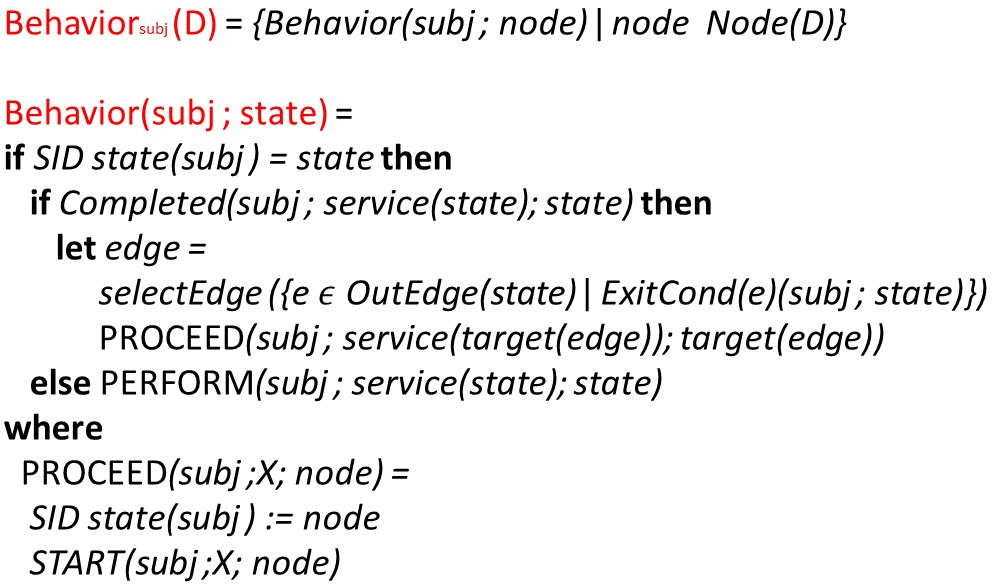
\includegraphics[width=0.7\linewidth]{20181026-Ontologie-Bilder/Grafiken-Ontologie/SUbjectExecution/ASM-Behavior}
%	\caption[Subject Behavior Diagram Interpretation]{Subject Behavior Diagram Interpretation}
%	\label{fig:asm-behavior}
%\end{figure}
%
%
%
%\section{Alternative Send/Receive Round Interpretation}
%
%\begin{figure}[ph]
%	\centering
%	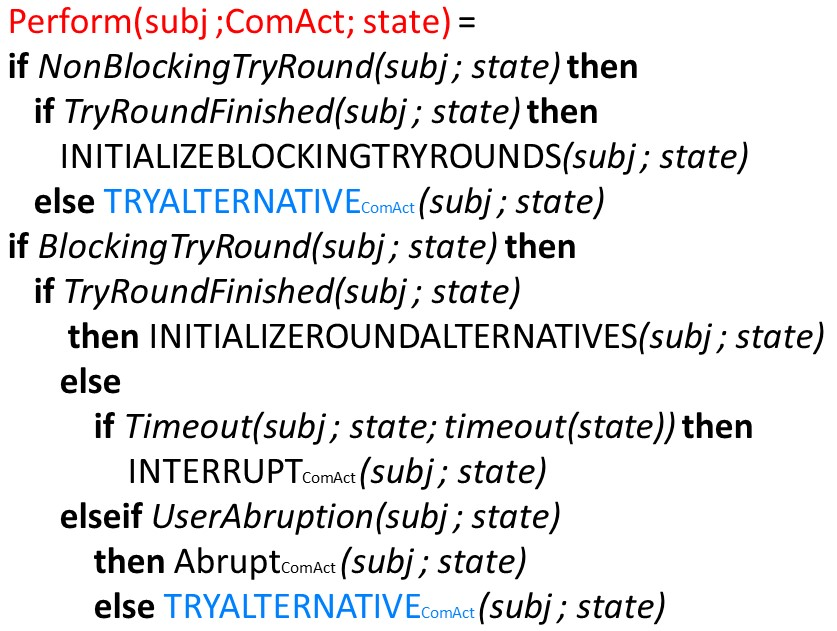
\includegraphics[width=0.6\linewidth]{20181026-Ontologie-Bilder/Grafiken-Ontologie/SUbjectExecution/ASM-perform}
%	\caption[Alternative Send/Receive Round Interpretation]{Alternative Send/Receive Round Interpretation}
%	\label{fig:asm-perform}
%\end{figure}
%
%\begin{figure}[ph]
%	\centering
%	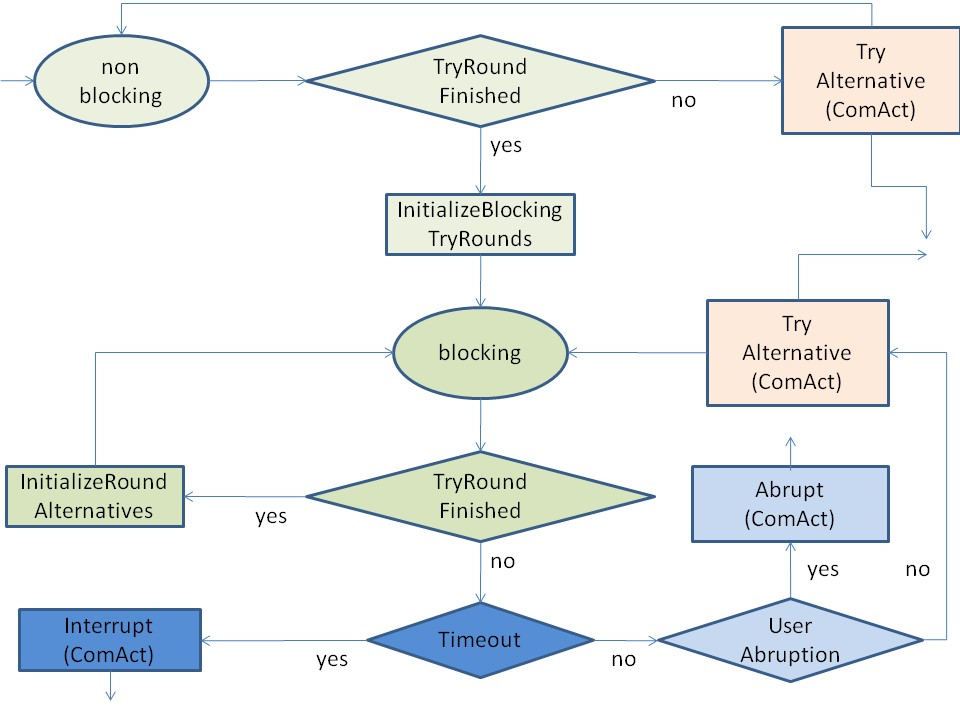
\includegraphics[width=0.6\linewidth]{20181026-Ontologie-Bilder/Grafiken-Ontologie/SUbjectExecution/ASM-Perform-Bild}
%	\caption[Diagram of Alternative Send/Receive Round Interpretation]{Diagram of Alternative Send/Receive Round Interpretation}
%	\label{fig:asm-perform-bild}
%\end{figure}
%
%\newpage
%\textbf{Interpretation of Auxiliary Macros}
%\begin{figure}[ph]
%	\centering
%	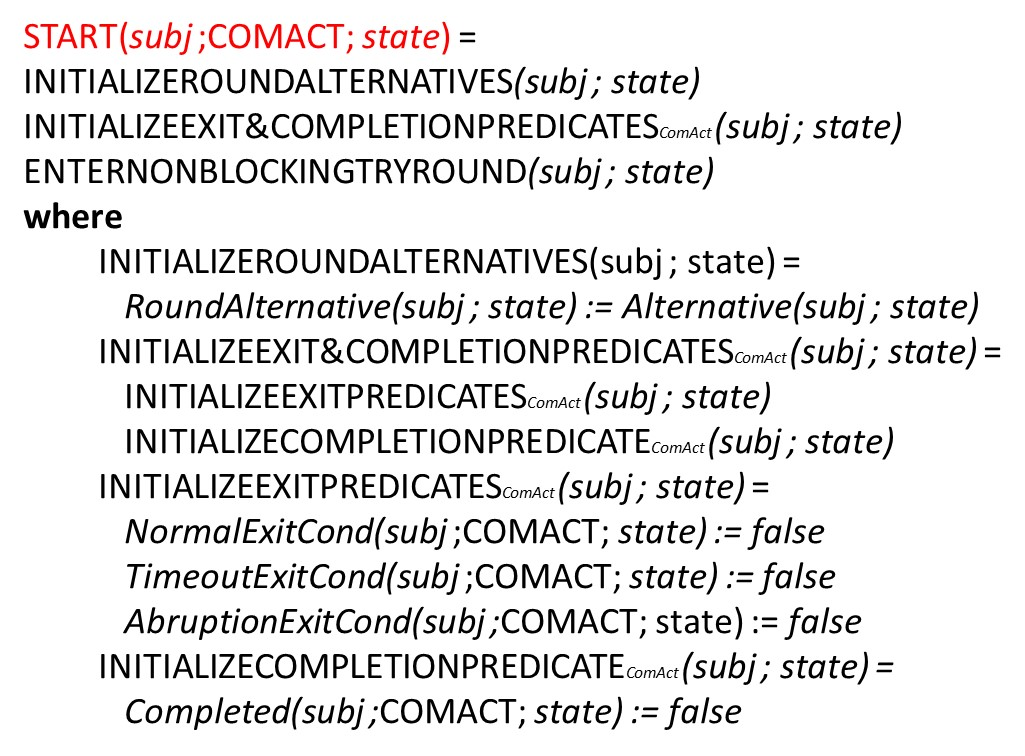
\includegraphics[width=0.7\linewidth]{20181026-Ontologie-Bilder/Grafiken-Ontologie/SUbjectExecution/ASM-Start}
%	\caption[Start function]{Start function}
%	\label{fig:asm-start}
%\end{figure}
%
%\begin{figure}[ph]
%	\centering
%	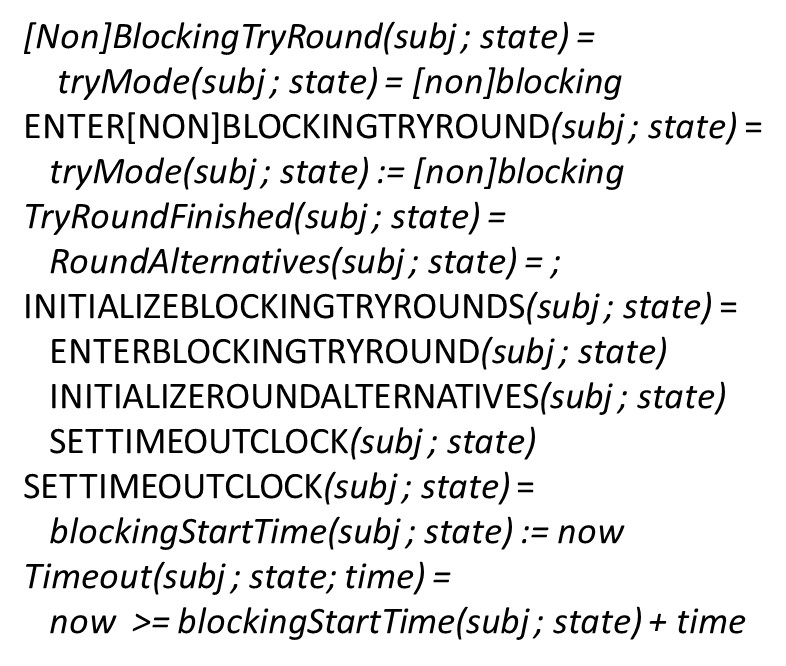
\includegraphics[width=0.6\linewidth]{20181026-Ontologie-Bilder/Grafiken-Ontologie/SUbjectExecution/ASM-Try-Run}
%	\caption[Try non/blocking Round]{Try non/blocking Round}
%	\label{fig:asm-try-run}
%\end{figure}
%
%\begin{figure}[ph]
%	\centering
%	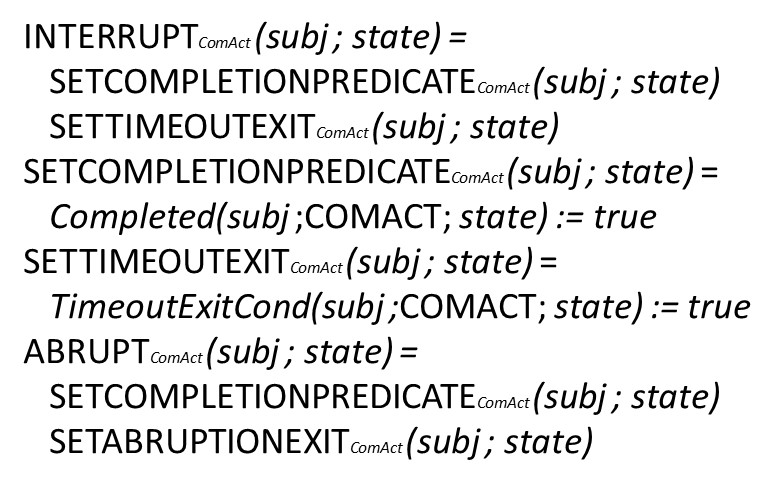
\includegraphics[width=0.6\linewidth]{20181026-Ontologie-Bilder/Grafiken-Ontologie/SUbjectExecution/ASM-Interrupt}
%	\caption[Interupt Handling]{Interupt Handling}
%	\label{fig:asm-interrupt}
%\end{figure}
%
%\newpage
%
%
%\section{MsgElaboration Interpretation for Multi Send/Receive}
%
%
%
%\section{Multi Send/Receive Round Interpretation}
%
%\section{Actual Send Interpretation}
%
%\section{Actual Receive Interpreation}
%
%
%\section{Alternative Action Interpretation}
%
%
%\section{Interrupt Behavior}
%
%
%\chapter{PASS Interpreter defined as Abstract State Machine (ASM)}
%
%\textbf{Class}\\
%\textbf{\emph{Object property}}\\
%\textit{ASM interpreter Specification}\\
%
%
%\begin{landscape}
%	\begin {longtable} {| p{0.5\textwidth} | p{0.3\textwidth} | p{0.6\textwidth}|}
%	\hline
%	OWL Model element &   ASM interpreter & Description\\
%	\toprule
%	\endhead
%	\hline
%	
%	X - Execution concept – the state the subject is currently in as defined by a \textbf{State} in the model & \textit{SID\_state} &  Execution concept – no model representation, Not to be confused by a model “state” in an SBD Diagram. State in the SBD diagram define possible SID\_States.
%	\\
%	\hline
%	
%	\textbf{SubjectBehavior }	– under the assumption that it is complete and sound.
%	& \textit{D} 
%	&  A Diagram that is a completely connected SBD
%	\\
%	\hline
%	
%	\textbf{State}
%	& \textit{node} 
%	&  A specific element of diagram D -	Every node 1:1 to state
%	\\
%	\hline
%	
%	\textbf{State}
%	& \textit{state} 
%	& The current active state of a diagram determined by the nodes of Diagram D
%	\\
%	\hline
%	
%	\textbf{InitialStateOfBehavior, \newline EndState }
%	& \textit{initial state, \newline end state} 
%	& The interpreter expects and SBD Graph D to contain exactly one initial (start) state and at least one end state.
%	\\
%	\hline
%	
%	\textbf{Transition}
%	& \textit{edge / outEdge} 
%	& “Passive Element” of an edge in an SBD-graph
%	\\
%	\hline
%	
%	\textbf{TransitionConditionn}
%	& \textit{ExitCondition} 
%	& Static Concept that represents a Data condition
%	\\
%	\hline
%	
%	Execution Concept – ID of a Subject Carrier responsible possible multiple Instances of according to specific  \textbf{SubjectBehavior}
%	& \textit{subj} 
%	& Identifier for a specific Subject Carrier that may be responsible for multiple Subjects
%	\\
%	\hline
%	
%	Represented in the model with \textbf{InterfaceSubject}
%	& \textit{ExternalSubject} 
%	& A representation of a service execution entity outside of the boundaries of the interpreter
%	(The PASS-OWL Standardization community decided on the new Term of Interface Subject to replace the often-misleading older term of External Subject)
%	
%	\\
%	\hline
%	\textbf{SubjectBehavior} or rather \textbf{SubjectBaseBehavior} as MacroBehaviors and GuardBehaviors are not covered by Börger
%	& \textit{subject-SBD / \newline SBDsubject\textsubscript{subject}} 
%	& Names for completely connected graphs / diagrams representing SBDs
%	\\
%	\hline
%	
%	Object Property: \textbf{\textit{hasFunctionSpecification}} 
%	(linking \textbf{State}, and \textbf{FunctionSpecification} -->(\textbf{State} \textbf{\textit{hasFunctionSpecification }} \textbf{FunctionSpecification})
%	& \textit{service(state) / \newline service(node)} 
%	& Rule/Function that reads/returns the service of function of a given state/node
%	\\
%	\hline
%	
%	\textbf{DoState} \newline \textbf{SendState} \newline \textbf{ReceiveState}
%	& \textit{function state, \newline send state, \newline receive state} 
%	& The ASM spec does not itself contain these terms. The description text, however, uses them to describe states with an according service (e.g. a state in which a (ComAct = Send) service is executed is referred to as a send state)
%	Seen from the other side: a SendState is a state with service(state) = Send)
%	\newline
%	Both send and receive services are a ComAct service.
%	The ComAct service is used to define common rules of these communication services.
%	
%	\\
%	\hline
%	\textbf{CommunicationActs} with sub-classes (\textbf{ReceiveFunction SendFunction}) \newline
%	\textbf{\textit{DefaultFunctionReceive1\_EnvironmentChoice \newline
%			DefaultFunctionReceive2\_AutoReceiveEarliest \newline
%			DefaultFunctionSend }}
%	& \textit{ComAct} 
%	& Specialized version of Perform-ASM Rule for communication, either send or receive. These rules distinguish internally between send and receive.
%	\\
%	\hline
%	
%	
%\end{longtable}
%\end {landscape}
%


